\documentclass{article}
\usepackage{graphicx, xcolor} % Required for inserting images
\usepackage[shortlabels]{enumitem}
\usepackage{amsfonts} 
\usepackage{amsmath}
\usepackage{graphicx}
\title{Deep learning HW 1}
\author{wbg231 }
\date{September 2023}

\begin{document}

\maketitle

\section{theroy}
\subsection{two layer neural networks}
\subsubsection{Regression task}
\begin{enumerate}[(a)] % (a), (b), (c), ...
\item (1pt) Name and mathematically describe the 5 programming steps you would take to train this model with PyTorch using SGD on a single batch of data
\begin{itemize}
    \color{blue}
    \item pass the input $x_i$ through the model $F$ to produce our prediction $\tilde{y}^{(i)}=F(x_i)$
    \item compute the loss $L(\tilde{y}^{(i)}, y^{(i)})$ between our prediction $\tilde{y}^{(i)}$ and the true value $y^{(i)}$
    \item compute the gradient of our loss function accumulated over all parameters $\nabla_{\theta}=\sum_{\theta_i}\frac{\partial L}{\partial \theta_i}$
    \item update our model parameters $\theta \leftarrow \theta - \eta \nabla_{\theta}L(\tilde{y}^{(i)}, y^{(i)})$
    \item zero our gradient $\nabla_{\theta}L(\tilde{y}^{(i)}, y^{(i)})\leftarrow 0$ 
\end{itemize}
\item (4pt)For a single data point(x,y),write down all inputs and outputs for forward pass of each layer. You can only use variable $x,y,W^{(1)},b^{(1)},W^{(2)},b^{(2)}$ in your answer. (note that $ Linear_i(x)=W^{(i)}x+b^{(i)}) $.
\begin{itemize}
    \color{blue}
    \item our input $x^i$ is passed to our first linear layer to produce $s^{1} = W^{(1)}x^{i} + b^{(1)}$
    \item $s^{(1)}$ is then passed to our first activation function f to produce $a^{(1)}=f(s^{(1)})=5reLU(s^{1})$
    \item $a^{(1)}$ is then passed to our second linear layer to produce $s^{(2)}=W^{(2)}a^{(1)}+b^{(2)}$
    \item $s^{(2)}$ is then passed to our second activation function g to produce our final prediction $\tilde{y}^{(i)}= I(s^{(2)})=s^{(2)}$
    \item our prediction $\tilde{y}^{(i)}$ is finally compared against the true value of example i $y^{(i)}$ to produce our loss $L(\tilde{y}^{(i)}, y^{(i)})=||\tilde{y}^{(i)}-y^{(i)}||_2$
    \item and those our the steps of this networks forward pass.
\end{itemize}
\item write down the gradients from the backwards pass. 
\begin{itemize}
   \color{blue}
    \item first we want to find $\frac{\partial C}{\partial \bold{W^2}}=\frac{\partial C}{\partial \bold{\tilde{y}}}\frac{\partial \bold{\tilde{y}}}{\partial \bold{s^2}}\frac{\partial \bold{s^2}}{\partial \bold W^2}=a^{2^t} 2(\tilde{y}-y)\in \mathbb{R}^{d\times k} $ where $W^2\in \mathbb{R}^{k\times d}$
    \item next we want $\frac{\partial C}{\partial \bold{W^2}}=\frac{\partial C}{\partial \bold{\tilde{y}}}\frac{\partial \bold{\tilde{y}}}{\partial \bold{s^2}}\frac{\partial \bold{s^2}}{\partial \bold b^2}=2(\tilde{y}-y)*1=2(\tilde{y}-y)^t\in \mathbb{R}^{1\times k } $
    \item then we want $\frac{\partial c}{\partial \bold b^1}= \frac{\partial C}{\partial \bold{\tilde{y}}}\frac{\partial \bold{\tilde{y}}}{\partial \bold{s^2}}\frac{\partial \bold{s^2}}{\partial \bold a^1}\frac{\partial \bold{a^1}}{\partial \bold z^1}\frac{\partial \bold{z^1}}{\partial \bold b^1}=2(\tilde{y}-y)W^{2}\frac{\partial \bold{ z^1}}{\partial \bold{a^1}}$
    \item \item then we want $\frac{\partial c}{\partial \bold W^1}= \frac{\partial C}{\partial \bold{\tilde{y}}}\frac{\partial \bold{\tilde{y}}}{\partial \bold{s^2}}\frac{\partial \bold{s^2}}{\partial \bold a^1}\frac{\partial \bold{a^1}}{\partial \bold z^1}\frac{\partial \bold{z^1}}{\partial \bold a^1}=2(\tilde{y}-y)W^{2}\frac{\partial \bold{ z^1}}{\partial \bold{a^1}}x $
\end{itemize}
\item show the elements of $\frac{\partial a_{1}}{s_{1}}, \frac{\tilde{y}}{s_2}, \frac{\partial C}{\partial \tilde{y}}$
\begin{itemize}
    \color{blue}
\item $\frac{\partial \bold{a^{1}}}{\partial \bold{s^{1}}}_{i}=\begin{cases}
            5& \text{if }s^{1}_{i} > 0 \\
            0 & \text{if }s^{1}_{i} < 0 \text{else}
            \end{cases}\in \mathbb{R}^{D}$
    \item now suppose that we know that $\tilde{y}\in \mathbb{R}^{K}$ and $s_2\in \mathbb{R}^{K}$ then we can see that $\frac{\partial \tilde{y}}{s_2}\in \mathbb{R}^{K}$ and $\frac{\partial \tilde{y}}{\partial s_2}=\frac{\partial s^{2}}{s^{2}} = I\in \mathbb{R}^{K} $ thus we can see that $\frac{\partial \tilde{y}}{s_2}_{i,j}=1\in \mathbb{R}^{k}$
    \item finally we can see that $C\in \mathbb{R}$ and $\tilde{y}\in \mathbb{R}^{k}$ thus $\frac{\partial C}{\partial \bold{\tilde{y}}}\in \mathbb{R}^{1\times K}$ and $\frac{\partial C}{\bold{\tilde{y}}}=\frac{\partial}{\partial \bold{\tilde{y}}}||y-\tilde{y}||_{2}=\frac{\partial}{\partial \tilde{y}}(y-\tilde{y})^{t}(y-\tilde{y})=-2(y-\tilde{y})^{t}$ thus we can see that $\frac{\partial C}{\partial \bold{\tilde{y}}}_{i}=-2(y-\tilde{y})_{i}$
\end{itemize}
\subsubsection{Classification task}
\begin{enumerate}
    \item If you want to train this network, what do you need to change in the equations of (b), (c) and (d), assuming we are using the same squared Euclidean distance loss function
   \begin{itemize}
    \color{blue}
    \item  we need to change our forward pass in the following ways.
    \begin{itemize}
        \item set our first layer activation function to be $f(s^{1})=tanh(s^{1})$
        \item set our second layer activation function to be $\sigma(s^2)=\frac{1}{1+e^{-s^{2}}}$
    \end{itemize}
    \item we also need to change our backward pass in the following ways.
    \begin{itemize}
        \item change $\frac{\partial a^ {1}}{\partial s^{1}}=\frac{\partial f}{\partial s^{1}}=\frac{\partial }{\partial s^{1}}tanh(s^1)=\frac{\partial }{\partial s^{1}}\frac{sinh(s^{1})}{cosh{s^1}}=1-tanh^{2}(s^{1})$
        \item also change $\frac{\partial  \tilde{y}}{\partial s^{2}}=\frac{\partial }{\partial s^{2}}(\sigma(s^{2}))=\frac{\partial }{\partial s^{2}}(\frac{1}{1+e^{-s^{2}}})=\frac{e^{-s^{2}}}{((1+e^{-s^{2}})^2)}=\sigma(s^{2})(1-\sigma(s^{2}))$
    \end{itemize}
    \item the following things change in the elements of our gradients
    \begin{itemize}
        \item we have $a^{1}\in \mathbb{R}^{D}, s^{1}\in \mathbb{R}^{d}$ $\frac{\partial \bold{a^{1}}}{\partial \bold{s^{1}}}\in \mathbb{R}^{d}$ where $\frac{\partial a^{1}}{\partial s^{1}}_{i} = \begin{cases}
            1-tanh^{2}(s^{1}_{i})
        \end{cases}$
        \item similarly we have $\tilde{y}\in \mathbb{R}^{k}, s^{2}\in \mathbb{R}^{k}$ meaning that $\frac{\partial \bold{\tilde{y}}}{\partial \bold{s^{2}}}\in \mathbb{R}^{k}$ and $\frac{\partial \tilde{y}}{\partial s^{2}}_{i} = \begin{cases}
            \sigma(s^{2}_{i})(1-\sigma(s^{2}_{i}))
        \end{cases}$
    \end{itemize}
   \end{itemize} 
\item Now you think you can do a better job by using a Bi- nary Cross Entropy (BCE) loss function $\ell(y,\tilde{y})=\frac{1}{K}\sum_{i=1}^{k}-[y_ilog(\tilde{y}_i) + (1-y_i)log(1-\tilde{y}_i)]$What do you need to change in the equations of (b), (c)
and (d)?
\begin{itemize}
    \color{blue}
    \item in our forward pass we need to make the following change 
    \begin{itemize}
        \item set $C(y,\tilde{y}) = \frac{1}{K}\sum_{i=1}^{k}-[y_ilog(\tilde{y}_i) + (1-y_i)log(1-\tilde{y}_i)]$
    \end{itemize}
    \item in the backwards pass we need to make the following change
    \begin{itemize}
        \item set $\frac{\partial C}{\partial \tilde{y}}=\frac{\partial }{\partial \tilde{y}}\frac{1}{K}\sum_{i=1}^{k}-[y_ilog(\tilde{y}_i) + (1-y_i)log(1-\tilde{y}_i)]=-\frac{1}{k}(N_1\sum_{y_i=1}\frac{1}{\tilde{y}}-(K-N_1)\sum_{y_i\neq 1}\frac{1}{1-\tilde{y}} ) $ where $N_1$ is the number of samples of class one. 
        \item this can also be expressed as $\frac{\partial c}{\partial \bold{y}}= -(\frac{y}{\tilde{y}}- \frac{1-y}{1-\tilde{y}})$
        \item the rest of our computation does not change from the last part as long as we update the above variable 
    \end{itemize}
\item finally the elements of our gradients can be changed as 
\begin{itemize}
    \item  $C\in \mathbb{R}, \tilde{y}\in \mathbb{R}^{K}, \frac{\partial \tilde{y}}{\partial \tilde{y}}\in \mathbb{R}^{1\times K}$ and we also have $\frac{\partial C}{\partial \tilde{y}}_{i} = \begin{cases}
        -\frac{1}{k}\frac{N_1}{\tilde{y}_{i}}& \text{if }y_i=1 \\
        \frac{1}{k}\frac{K-N_1}{1-\tilde{y}_{i}} & \text{if }y_i\neq 1
        \end{cases}=-(\frac{y}{\tilde{y}}- \frac{1-y}{(1-\tilde{y})})$
        \item $\frac{\partial \tilde{y}}{\partial s^2}=\frac{e^{-s^2}}{(1-e^{s^2})^2}$
        \item $\frac{\partial a^1}{\partial s^1} =1-tanh(s^1)^2$
    \end{itemize}
\end{itemize}
\item (1pt) Things are getting better. You realize that not all intermediate hidden activations need to be binary (or soft version of binary). You decide to use $f (*) = (*)^+$ but keep g as $\sigma$. Explain why this choice of f can be beneficial for training a (deeper) network.
\begin{itemize}
    \color{blue}
    \item suppose we have a deep neural network, and two examples $x_i, x_j$ such that we are quite confidante (say we know it 100\%) in the Classification of $x_i$  and only fairly confidante in the Classification of $x_j$ say we are only \%75 sure, in a binary or soft binary activation function these two examples will have a similar output that is $s^1(x_j)\approx s^1({x_i})$, then these $s^{1}$ values are passed onto the second layer of the network with little to no information about how confidante our previous layer was. You can intuitively understand how over many layers this could lead our networks activations to become distorted
\end{itemize}
\end{enumerate}
\end{enumerate}
\subsection{Conceptual Questions}
\begin{enumerate}[(a)]
    \item why is the softmax function really softmaxarg function
    \begin{itemize}
        \color{blue}
        \item the soft max function is defined as $\sigma(x_i)=\frac{e^{x_i}}{\sum_{i}e^{x^{i}}}$ so intuitively what this function is doing is normalizing our our network outputs be all positive and sum to one. in this way we can think of them as probabilities. 
       \item thus if we are using the softmax in a Classification we will predict the class with the highest probability ie (assuming index class labels) $\tilde{y}=argmax_{i}\sigma(x_i)$
    \end{itemize}
    \item draw the computation graph
    \begin{itemize}
        \color{blue}
        \item 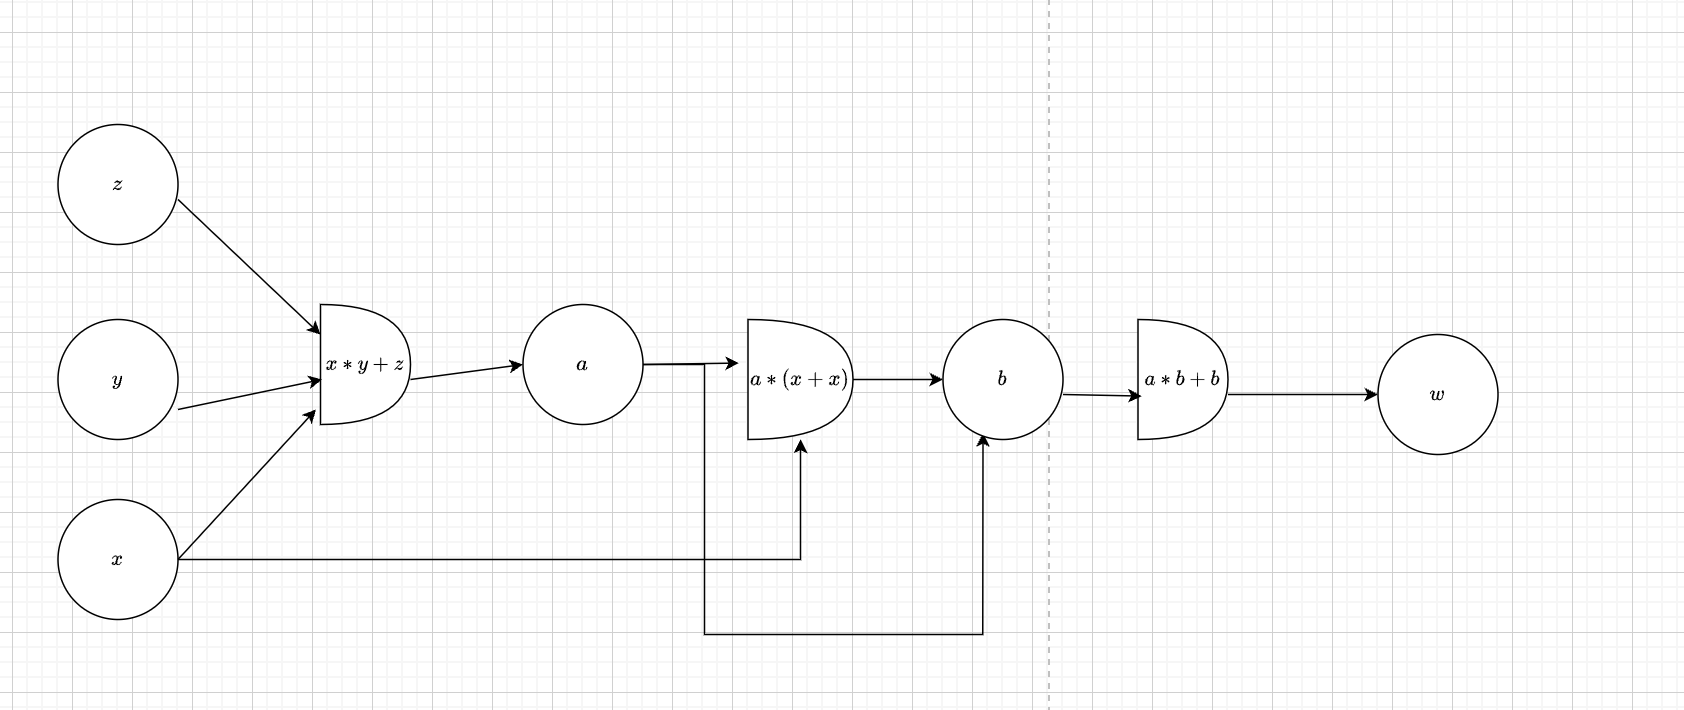
\includegraphics[scale=.5]{./figs/question_1_2_b.png}
    \end{itemize}
    \item draw the graphs 
    \begin{itemize}
        \color{blue}
        \item 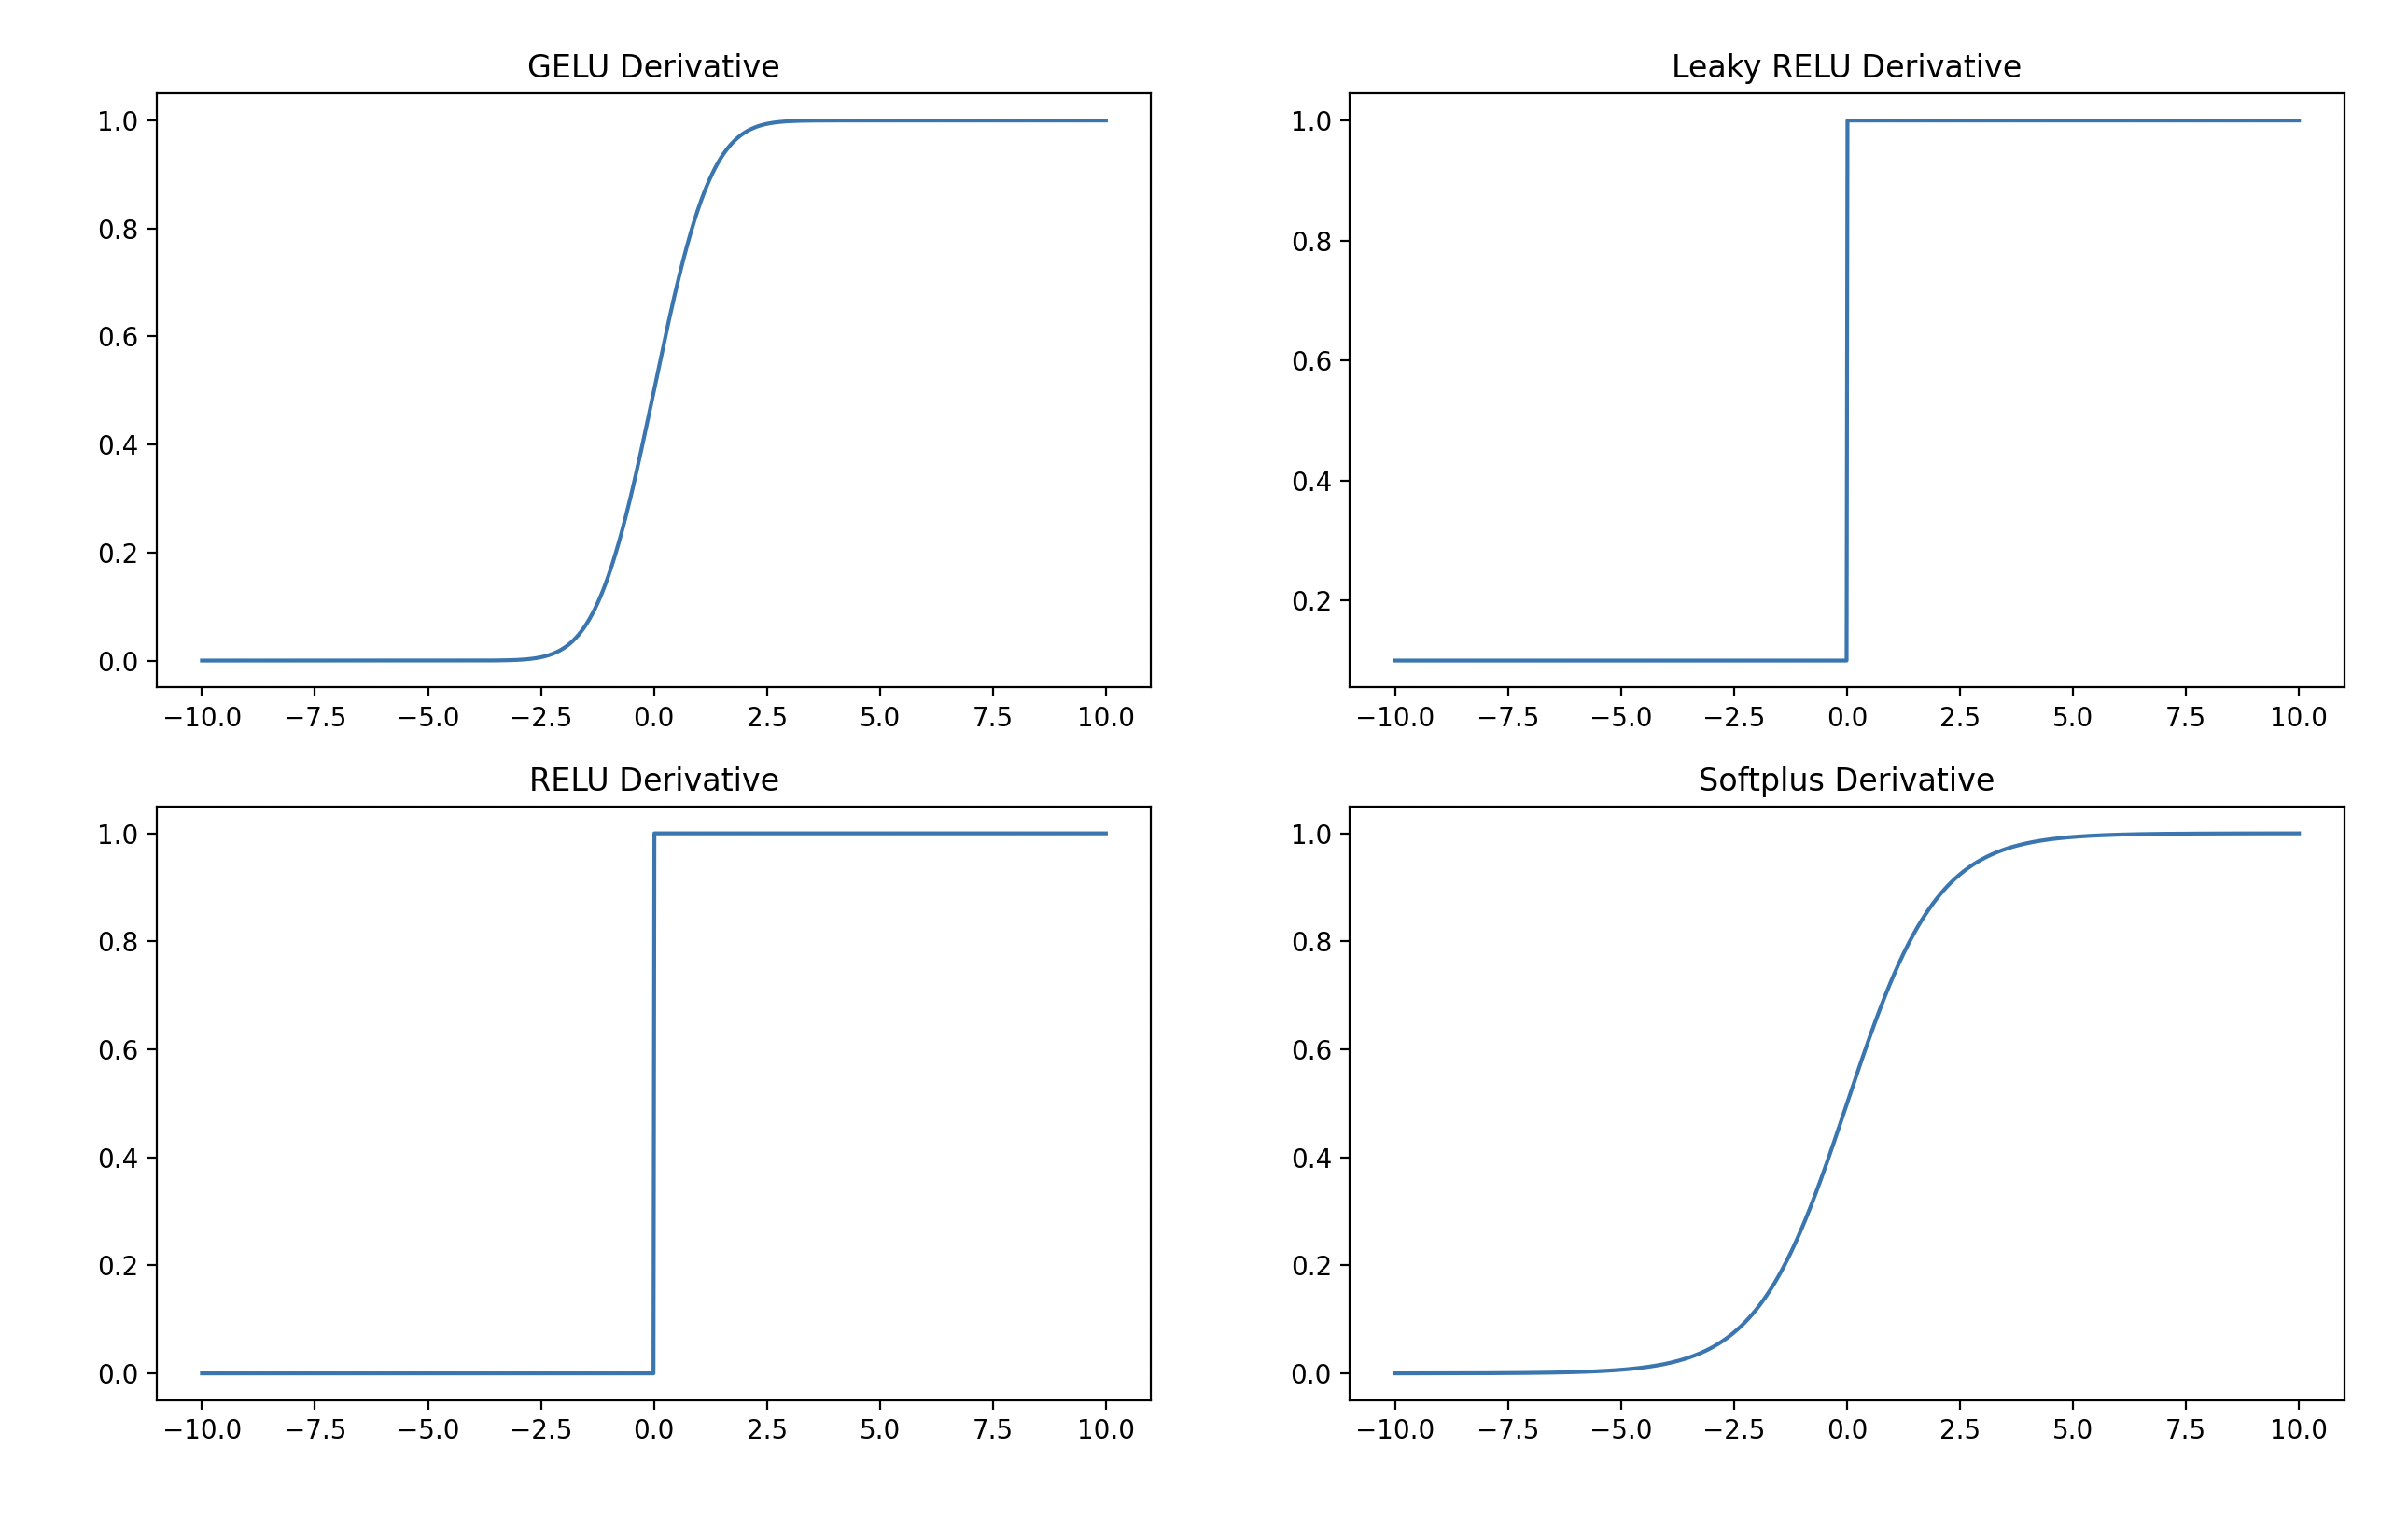
\includegraphics[scale=.3]{./figs/question_1_2_c.png}
    \end{itemize}
    \item given the functions $f(x)=W^{1}x, g(x)=W^{2}x:\quad W^1\in \mathbb{R}^{b\times a}, W^{2}\in \mathbb{R}^{b\times A}$
    \begin{enumerate}[(a)]
        \item what are the gradients of $f$ and $g$ with respect to $x$?
        \begin{itemize}
           \color{blue}
            \item we can see that $\frac{\partial f}{\partial x}=W^{1}\in \mathbb{R}^{b\times a}$ and $\frac{\partial g}{\partial x}=W^{2}\in \mathbb{R}^{b\times A}$
            \item thus our jacobians are $\nabla_f(x)=W^1, \nabla_g(x)=W^2$
        \end{itemize}
    \item what is the gradient of $h(x)=f(x)+g(x)$

    \begin{itemize}
        \color{blue}
        \item we know that differentiation is a linear operation thus $\frac{\partial h}{\partial x}=\frac{\partial}{\partial x}(f(x)+g(x))=\frac{\partial}{\partial x}(f(x))+\frac{\partial}{\partial x}(g(x))=W^{1}+W^{2}$
        \item thus our jacobian is $\nabla_h(x)=W^1+W^2$
    \end{itemize}
    \item what is the gradient of $h(x)=f(x)+g(x) \text{ when } W^1=W^2$

    \begin{itemize}
    \color{blue}
    \item using what we showed above we know $\frac{\partial h}{\partial x} = W^1+W^2=2W^1=2W^2 $
    \item thus our jacobian is $\nabla_h(x)=2W^1=2W^2$
\end{itemize}   
\end{enumerate}
\item given the functions $f(x)=W^{1}x, g(x)=W^{2}x:\quad W^1\in \mathbb{R}^{b\times a}, W^{2}\in \mathbb{R}^{c\times b}$
\begin{enumerate}[(a)]
    \item what are the gradients of $f$ and $g$ with respect to $x$?
    \begin{itemize}
       \color{blue}
        \item we can see that $\frac{\partial f}{\partial x}=W^{1}\in \mathbb{R}^{b\times a}$ and $\frac{\partial g}{\partial x}=W^{2}\in \mathbb{R}^{b\times A}$
        \item thus our jacobians are $\nabla_f(x)=W^1, \nabla_g(x)=W^2$
    \end{itemize}
\item what is the gradient of $h(x)=g(f(x))$

\begin{itemize}
    \color{blue}
    \item  by the chain rule we know that $\frac{\partial h}{\partial x}= \frac{\partial g}{\partial f}\frac{\partial f}{\partial x}$
    \item we know that $f(x)=W^1x\in \mathbb{R}^{b}$ is a vector so using what we showed above we can see  $\frac{\partial g}{\partial f}=\frac{\partial}{\partial f}W^{2}f=W^2$
    \item and also from what we showed above we have $\frac{\partial f}{\partial x}=W^1$
    \item so finally we can see that our jacobian matrix $\nabla_{h}(x)=W^2W^1$ meaning that $\nabla_h(x)_{i,j}=W^{2^t}_{i}W^{1}_j $
\end{itemize}
\item what is the gradient of $h(x)=g(f(x))$ if $W^1=W^2$
\begin{itemize}
\color{blue}
\item using what we showed above we know $\frac{\partial h}{\partial x} = W^1W^2=W^1W^2=W^2W^2$
\item thus our jacobian is $\nabla_h(x)=W^1W^1=W^2W^2$
\end{itemize}   
\end{enumerate}
    \end{enumerate}
\subsection{Deriving Loss Functions}
Derive the loss function for the following algorithms based on their common up- date rule $w_i \leftarrow w_i + \eta (y_i - \tilde{y}_i)x_i$Showthestepsofthederivationgiventhefollowing inference rules (simply stating the final loss function will receive no points).
\begin{enumerate}
    \item Perceptron: $\tilde{y}=sign(b+\sum_{i=1}^{d}w_ix_i)$
    \begin{itemize}
        \color{blue}
        \item from a geometric perspective we can see that the perceptron is trying to find a hyperplane that separates the data. our function makes a binary prediction of either 1 or -1 (corresponding to sides of the hyperplane).
        \item out update rule keeps our weight vector the same if the $\tilde{y}=y$, and if $y=1 \land \tilde{y}=-1$ moves $w_i$ in the direction of $x_i$ and if $y=-1 \land \tilde{y}=1$ moves $w_i$ in the direction of $-x_i$
        \item though our activation function $sign(*)$ is binary we would still like our predictions to be as confidant as possible. this confdince is reflected in the linear activation $b+\Sigma_{i=1}^{d}w_ix_i$
         thus we can see that our loss function should be a function of the distance between our prediction and the true value.
        \item so we would like a loss function that respects these facts as well as our learning rule  $w_i \leftarrow w_i + \eta (y_i - \tilde{y}_i)x_i$ meaning that for gradient descent to work we want $\nabla_c(w_i)= (y-\tilde{y})x_i$ 
        \item all of these conditions can most simply be achieved with $C(y,\tilde{y})=-(y-\Tilde{y})\sum_{i=1}^{d}x_iw_i$  which is the loss function we ultimately use for the perceptron.
        \item note however that this does not have to result in a unique hyperplane, any hyperplane which devides all of the points correctly result in a zero loss 
    \end{itemize}
    \item Adeline: $\tilde{y}=b+\sum_{i=1}^{d}x_iw_i$
    \begin{itemize}
        \color{blue}
        \item the Adeline is a Regression problem with an identity activation function.
        \item this is effectively linear Regression that is we can think of our weight vector w (and bias b) as the best linear function mapping $x_i$ to y 
        \item we can Conceptualize best in this case as meaning the minium Euclidean distance between our prediction and the true value.
        \item thus our cost function can be thought of as $\frac{1}{2}C(y,\tilde{y})=||y-\tilde{y}||_{2}$ or $\frac{1}{2}(y-\tilde{y})^{2}$ (or as a loss function $L(x_i,w_i,y)=\frac{1}{2}(y-(b+\sum_{i=1}^{d}x_iw_i))^2 $) 
        \item here we are adding the $\frac{1}{2}$ so the gradient of our cost function is the same as our update rule that is $-(y-\tilde{y})x_i$
        \item this will result in a unique solution for our weight vector w and bias b
    \end{itemize}
    \item Logistic Regression: $\Tilde{y}=tanh(\sum_{i=1}^{d}w_ix_i)$
    \begin{itemize}
        \color{blue}
        \item the tanh activation function (which is a shifted version of the sigmoid $tanh(x)=2\sigma(2x)-1$) scales our output to be between -1 and 1
        \item so we want a  cost function that is 0 when $y=\tilde{y}$ and increases as $y$ and $\tilde{y}$ diverge, and also respects our weight update rule $w_{i}\leftarrow w_i+\eta (y-\tilde{y})x_i$. 
        \item this loss function is given by $\ell(x_i,y,w_i)=-2log(1+e^{-y*w_i^tx_i})$. checking this is more or less just calculus at this point 
        \item note that this loss function is convex and thus has a unique solution for our weight vector w
        \item also note that this loss function is the same as the binary cross entropy loss function we derived in the previous section
        \item $\frac{\partial \tilde{y}}{\partial \bold{w}_i}=1-tanh^2(w^tx+b)x$
        \item $\frac{\partial \ell}{\partial \tilde{y}}=\frac{(\Tilde{y}-y)}{1-tanh^2(w^tx+b)}$
        \item then we can finally see that $L=\int\frac{\partial L}{\partial \tilde{y}}dy=\frac{\tilde{y}^2-y\tilde{y}}{2-2tanh(b+w^tx)}$
    \end{itemize}
\end{enumerate}
\end{document}
